\documentclass{article}
\usepackage[utf8]{inputenc}
\usepackage{fancyhdr}
\usepackage[margin=2.8cm,twoside]{geometry}
\usepackage[super]{nth}
\usepackage[english]{babel}
\usepackage{csquotes}

\usepackage{hyperref}
\usepackage[backend=biber,style=ieee]{biblatex}
\addbibresource{bibliography.bib}

\usepackage{float}

\pagestyle{fancy}
\fancyhf{}
\fancyhead[LE,RO]{DID - 04 Preliminary Design (Hebb \& Stephan)}
\fancyhead[LO,RE]{\leftmark}
\fancyfoot[LE,RO]{\thepage}

\usepackage{graphicx}

\begin{document}
	
\begin{titlepage}
	\begin{center}
		\vspace*{1cm}
		
		\LARGE\textsc{Royal Military College of Canada}\normalsize
		
		\vspace{0.2cm}
		
		\textsc{Department of Electrical and Computer Engineering}
		
		\vspace{1.5cm}
		
		
\includegraphics[width=0.3\textwidth]{rmcLogo.png}
		
		\vspace{1.5cm}
		
		\LARGE{Designing Coatimunde\\}
		
		\vspace{0.2cm}
		
		\normalsize{Computer Optics Analyzing Trajectories In Mostly Unknown, Navigation Denied, Environments}
		
		\vspace{0.1cm}
		
		\normalsize{DID-07 - Detailed Design Document}
		
		\vfill
		
		\textbf{Presented by:}\\Amos Navarre \textsc{Hebb} \& Kara \textsc{Stephan}\\
		\vspace{0.8cm}
		\textbf{Presented to:}\\Dr. Sidney \textsc{Givigi??} \& Anthony \textsc{Marasco} \& Dr. ?????? \textsc{??????} 
		\vspace{0.8cm}
		
		\today
		
	\end{center}
\end{titlepage}

% \begin{abstract}
% \end{abstract}


\tableofcontents

\newpage

\section{Introduction}

	\subsection{Document Purpose}
	
	Using Computer Optics for Analyzing Trajectories in Mostly Unknown, Navigation Denied, Environments (\textsc{coatimunde}) is the goal of this project. The purpose of this document is to outline the detailed design for \textsc{coatimunde}. That is, any deviations from the original design/plan, what the final design was, how it was built, and how this met the requirements of the project.  The requirements for the project have been outlined in the Statement of Requirements. This design of the project is shown, through design artefacts, and discussed in the Design Section. The final results of the project are presented in the Results section, and the tests done to obtain these results are presented in the Verification and Validation section. This document will then provide a summary of the degree of success of the project and provide feedback on the course experience as a whole.
	
	\subsection{Background}
	
	Both in the consumer and professional sectors the use of autonomous aerial vehicles is growing quickly. Currently these vehicles rely on skilled pilots to accomplish a very limited set of tasks. Adding obstacle avoidance capabilities to these vehicles and simplifying the task of following targets could allow for these systems to be used in many more situations. This section will give a quick background on obstacle avoidance, unmanned aircraft systems, computer vision, and the platforms we intend to use in this project.

		\subsubsection{Aim}
	
	The aim of this project was to design a high level control system that will allow an air robot to identify a target and move toward it, avoiding any obstacles that are in the way. Tracking targets of interest in complex environments with a flying robot was the ultimate goal of this project. To accomplish this goal we used a TurtleBot and then a flying robot through only the use of a camera to identify targets and obstacles. 
		
		\subsubsection{Benefits}
		
		Having a flying robot capable of accomplishing the project's tasks while totally autonomous will allow for the use of flying robots in environments closer to the ground, and will assist pilots in complex environments. These general requirements can be used in many situations. These benefits for society are the motivation behind this project.
		
		\begin{itemize}
			\item \textbf{Surveillance:} The robot could follow an interesting object, especially in an urban environment, without colliding with obstacles.
			\item \textbf{Search and Rescue:} The robot could move toward visual way-points set by pilots while avoiding obstacles in complex environments assisting in search efforts.
			\item \textbf{Inspections:} The robot could inspect objects in hard to reach environments and complex environments like rooftops or bridges.
			\item \textbf{Disaster Relief:} The robot could check inside buildings that may have compromised structural integrity, rubble on ground, \textit{\&c}.
			\item \textbf{Agriculture:} The robot could inspect tree-fruit or crops that can not be observed from overhead or check assets in remote locations such as irrigation equipment.
		\end{itemize}

		\subsubsection{Scope}
	
	The project started through the use of a ground robot then progressing to a flying robot. The project used computer vision to find targets and for avoiding multiple obstacles. Both robots are be highly autonomous, requiring only user input to commence. 

	The scope of the project was limited due to only being able to test indoors. Ideally the UAV would be operating at a high speed and identifying an arbitrary target in an unpredictable environment. In this case though the testing was completed within the confines of a relatively small robotics laboratory. Smaller obstacles were used indoors simply due to space constraints. Lower speeds were used as well, again due to the lack of space. 


		\subsubsection{Requirements}
	The requirements for the project are described in the Statement of Requirements (DID-03) \cite{sor}. The main functional requirements for this project were identification and movement towards a target within 15m radius, and identification and avoidance of multiple obstacles. CAN ADD MORE

		\subsubsection{Preliminary Design}
	The preliminary design document outlines out the initial design for the project \cite{pdd}. 
The original design has mostly remained the same for the large part but small details throughout the different aspects have changed to allow for functionality. ??? how to word?
	- what did the PD lay out and what remained the same from it? Overview

		\subsubsection{Changes to Schedule}

	- delay of getting the robot to identify targets and move towards them (REF schedule update) \cite{schupd}
	- change of the layout of custom nodes (can send them to design section for custom nodes?)
	- delay of porting to UAV

	\subsection{Definitions}
	- add more def if you want
	
		\subsubsection{Obstacle Avoidance}
		
		
		Obstacle avoidance is the task of satisfying a control objective, in this case moving toward a visual target, while subject to non-intersection or non-collision position constraints. The latter constraints are, in this case, to be dynamically created while moving in a reactive manner, instead of being pre-computed.
		
		\subsubsection{Unmanned Aircraft Systems}
		
		Very generally any powered vehicle that uses aerodynamic forces to provide lift, without a human operator being carried, can be considered an unmanned aerial vehicle. Currently most of these vehicles make up a single component of a larger unmanned aircraft system. An Unmanned aircraft system (UAS), or remotely piloted aircraft system (RPAS), is an aircraft without a human pilot on-board, instead controlled from an operator on the ground. Such a system can have varying levels of autonomy, something as simple as a model aircraft could be considered a UAS without any automation capabilities. 
		
		\subsubsection{Computer Vision}
		
		Currently there are many different ways that computers can make high-level decisions based on digital image information. There are many methods to acquire, process, and analyze data from the real world using a camera. While this is a very broad field, we intend to focus on motion estimation and object recognition. Both will be working with a video stream taken from a camera. 
		
		Motion estimation can be accomplished using direct methods which compare whole fields of pixels to each other over successive frames, compared to indirect methods which look for specific features. The information resulting from motion estimation streams can be used to both compensate for motion while analyzing other aspects of an image, and update a state machine.
		
		Object recognition in our project will be accomplishing two tasks: identifying a marker or target which will require more involved object recognition calculations, and very simple techniques, such as edge detection, to identify obstacles that exist in the path of the robot.
		
		\subsubsection{OpenCV}
		
		The Open Source Computer Vision Library (OpenCV) of programming functions is a cross-platform and free for use collection of functions primarily aimed at real-time computer vision\cite{opencv}. Most well documented techniques to accomplish all of the computer vision goals of our project have already been created and refined in OpenCV. For this reason this project utilized a lot of preexisting OpenCV functions.
		
		\subsubsection{Gazebo}
		
		Gazebo is a robot simulator that allows for creation of a realistic environment which includes both obstacles and markers similar to those being used in the lab. It was then used to rapidly test algorithms.
		
		\subsubsection{Robot Operating System}
		
		The Robot Operating System (ROS) is a distributed message system that allows for various sensors and processors to work together to control a robot. It is open source and has been integrated already with OpenCV and Gazebo. There are many additional tools for detecting obstacles, mapping the environment, planning paths, and much more. It is also a robust messaging system that has been proven to be capable of real-time processes.
		
		\subsubsection{TurtleBot}
		
		The TurtleBot is a robot kit with open-source design and software. A TurtleBot is a robot built to the specification for TurtleBot Compatible Platforms\cite{wise_foote_2011}. In this case the turtlebto has a Kobuki Base, an Acer Netbook running Ubuntu with ROS packages added, an X-Box Kinect, and some mounting plates. 
		
		The resulting robot looks like a disk supporting some circular shelves with a small laptop and a camera on the shelves. The base disk is 35.4cm in diameter, the topmost shelf is 42cm from the ground. The robot has a maximum speed of 0.65m/s. 
		
		\subsubsection{AscTec Pelican}
		
		The Ascending Technologies Pelican is a 65.1cm by 65.1cm quad-copter designed for research purposes\cite{asctec}. It includes a camera, a high level and low level processor set up for computer vision, and simultaneous localization and mapping (SLAM) research. It is also capable of interfacing easily with other controllers and can carry up to a kilogram of additional gear.






		
\section{Design}
	
	\subsection{Computer Vision}
	
	Computer optics was used as the robot employed a camera to identify objects in the surrounding environment, specifically targets and obstacles. There are three unique manners that computer vision was used as an input source for this project; these are target finding, obstacle finding, and optical flow. The implementation of all three created a navigation kit that uses exclusively a camera as input resulting in a very transferable and lightweight package for flying robots.
	
		\subsubsection{Target Finding}
		
		While finding arbitrary targets would be preferred, this project is going to be limited to finding special targets designed to be easily identified in a busy environment called ArUco shapes. There are existing libraries in OpenCV that are useful for identifying ArUco shapes with very little overhead. 
		
		\subsubsection{Obstacle Finding}
		
		Finding obstacles will be a considerable aspect of this project. There are various algorithms which leverage the robot's motion through the environment to extract key features of the environment, indicating the potential presence of obstacles. Parallax shift is the tendency for items that are closer to a camera to appear to move more or change in size more than a background that is further away and can be used to indicate where items are and how close they are. Occlusion is where one item moves in front of another item and covers it up, this indicates that the item still in view is closer to the camera than the item that has been hidden. OpenCV contains libraries for both of these tasks, as well as others that may end up being employed to identify obstacles in the environment.
		
		\subsubsection{Optical Flow}
		
		Optical Flow is a possible source of motion information for the robot. As a camera is moved through an environment the entire image will appear to scale larger as the camera moves forward, rotate left and right as a robot rolls, and shift left, right, up, and down as the robot pitches and yaws. Calculating shifts from one frame to another for global shifts caused by movement of the camera is a mathematically intensive process beyond the scope of this project. OpenCV contains libraries to try to parse this information, but it requires a considerable amount of effort to combine this information with a model of a robot to get useful position estimation.
	
	\subsection{Analyzing Trajectories}
	
	Analyzing trajectories is a term that refers to the robot completing movements to go towards the target. To do path planning the project will implement potential fields. Potential fields function through creating vectors pointing to objects in the environment and assigning them positive or negative. The positive vectors attracts the robot towards the target and the negative makes obstacles repulsive to the robot \cite{hwang1992potential}. This algorithm was selected to do path planning as the robot will not have to build a map of the environment to create path to the target \cite{bortoff2000path}. Potential fields allow for the robot to change its path along the way if it discovers new obstacles. As the robot is moving the potential fields must be updated to account for how much the robot moved. This will be solved through creating a state machine. 

	\subsection{Unknown and Navigation Denied Environments}

	The robot must always remember where identified target and obstacles are in relation to itself even when its own position changes. Navigation denied means that the robot will not have access to a GPS to locate itself, so it must search its unknown environment to identify targets and obstacles. An unknown environment can be defined as an environment in which the robot has no prior knowledge of its surroundings and must identify objects in this environment itself through computer vision. Potential fields will be used to track the location of the target and obstacles through updating each objects vector. These vectors will be used in the state machine to properly create a path to the target, as they are either negative for the target or positive for obstacles. This once again is the reason that the project will be using potential fields to plan the path to the target. 


	\subsection{Block Diagram}
	
	The block diagram that is shown in Figure \ref{fig:blockdiagram} contains the outline of the \textsc{coatimunde} project. It is a very high level overview and does not contain references to most of the hardware in use for two reasons: the actual robot and laptop being used are relatively arbitrary as long as the software included is present on both. ROS also includes many nodes which are not represented on the block diagram. Only the nodes that are most important to our project, will have to be specifically added to ROS, or will have to be custom created are included on our system block diagram shown below.
	
	The laptop contains the initialization, target selection, and RViz. The laptop also takes the user input when necessary and processes it appropriately.  The robot will do all the target identification, obstacle avoidance, and movement decisions autonomously. This means it will take input from the camera into a video processing node and then create a corresponding ROS message to be sent to the other systems on the robot. These messages are created and used throughout the different systems on the robot. The model of the robot's environment will be found subscribing to messages from the obstacle finder node, target finder node, and the state estimate node. This model then creates a message to pass to the route planning node which tells the movement node how to update its position and speed. 
	
	Most of the nodes used in this project are either being used stock, or are very minimally modified from provided libraries. The four nodes, highlighted in grey, which are being custom built for this project are the State Estimate, Target Finder, and Obstacle Finder. 

	\begin{figure}[H]
		\centering
		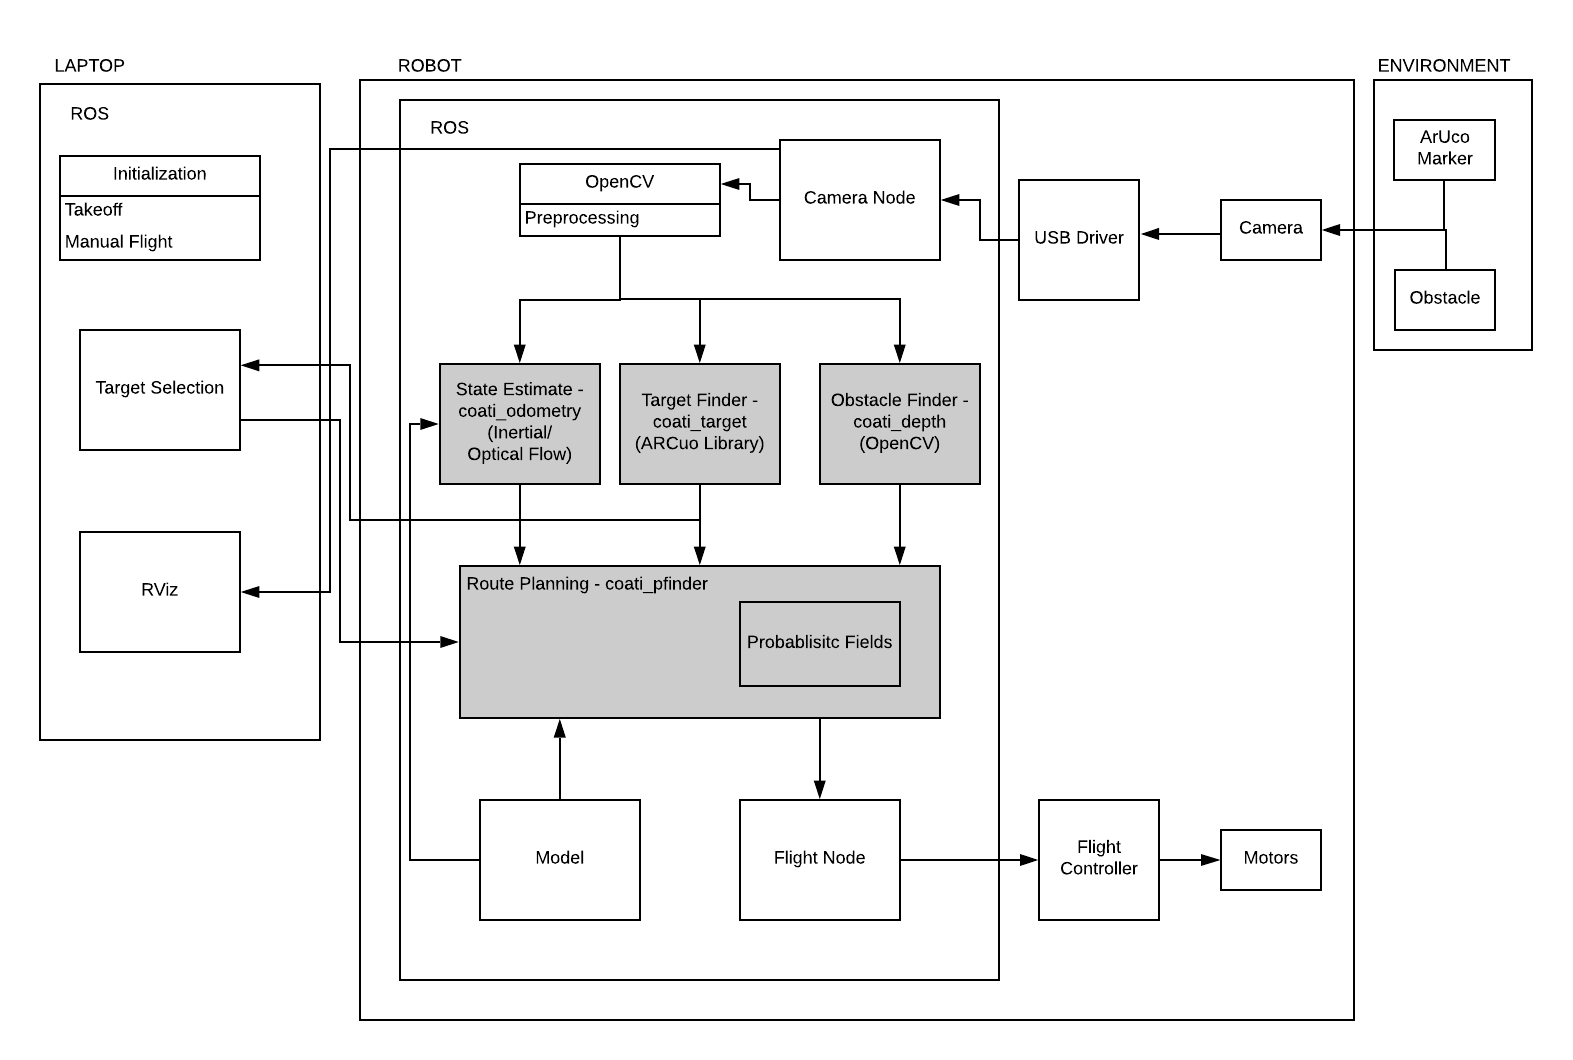
\includegraphics[width=\linewidth]{BlockDiagram}
		\caption{Project Block Diagram}
		\label{fig:blockdiagram}
	\end{figure}

	\subsection{Custom Nodes}
	
	 All of the nodes being written for this project will be written in Python and then built in ROS to be implemented on the robot. Python is being used for this project because C++ and Python are the most supported languages for both ROS Nodes and OpenCV. While C++ could possibly be faster in execution, we believe that most of our bottlenecks will be in the actual processing of images. The library calls to OpenCV will still be executing in the lower level C that OpenCV is written in, so there would be minimal gains to be had writing in C++.
	 
	 The Camera node is referenced in many locations. The camera node is built in to ROS and provides image data in various formats. Processes can to subscribe to different image formats. In general the raw image information will be used by the other nodes. Common transformations that must be applied to all functions these will be done in the common camera node to avoid unnecessary calculations.
	
	\subsubsection{Target Finding}
	
	\begin{figure}[H]
		\centering
		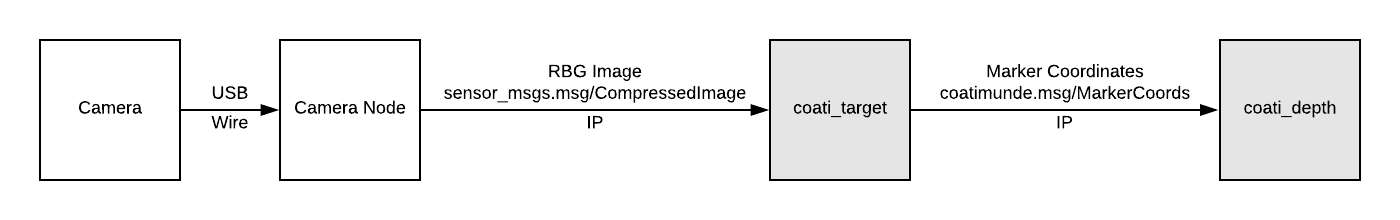
\includegraphics[width=0.9\linewidth]{TargetDiagram.png}
		\caption{Target Finding Node}
		\label{fig:target}
	\end{figure}

	Camera data, after being processed by the camera node, goes into the target finder node. The target finder is mostly implementing the ArUco symbol finding libraries in OpenCV. ArUco symbols are intended for augmented reality purposes and provide very accurate position, orientation, and distance information. These values will be translated into a vector value that the other systems on the robot can understand and be published at least 10 times per second.
	
	Given the limited field of view of the robot it may not always be able to see the target, in which case it will continue to scan for targets.
	
	ArUco markers normally encode simple ID information. Vectors will carry the same identifiers allowing the route planning parts of the robot to know when a target has been re-spotted and over-write it or allow for finding and remembering the positions of multiple targets. 
	
	\subsubsection{Obstacle Finding}
	
	\begin{figure}[H]
		\centering
		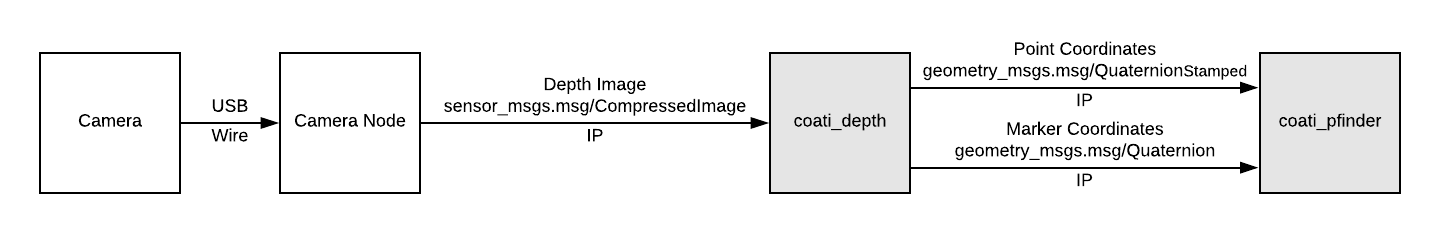
\includegraphics[width=0.9\linewidth]{DepthDiagram.png}
		\caption{Obstacle Finding Node}
		\label{fig:obstacle}
	\end{figure}

	Finding obstacles with depth information will be difficult using monocular vision. The current plan is to try to combine parallax shift with edge detection to try to parse information about nearby objects. These vectors will be published as a large ROS message at least 10 times per second. 
	
	Getting depth information from a single camera is difficult. The TurtleBot also has a suite of depth sensors built in with the camera so these may be used initially instead of trying to use parallax information from a camera to allow for testing other aspects of the system.
	
	\subsubsection{State Estimator}
	
	\begin{figure}[H]
		\centering
		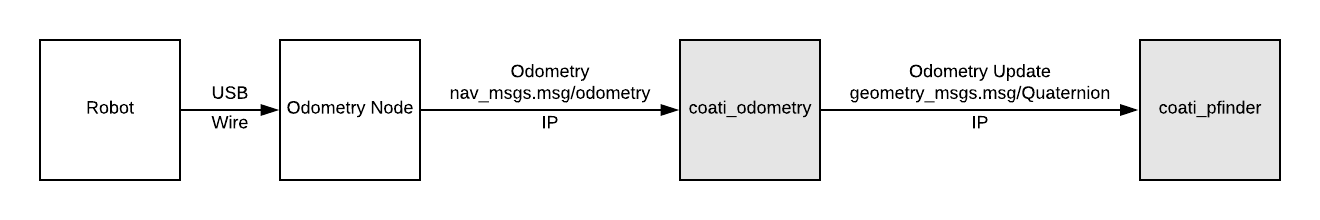
\includegraphics[width=0.9\linewidth]{OdometryDigram.png}
		\caption{State Estimating Node}
		\label{fig:state}
	\end{figure}

	State estimating from camera information is very difficult and computationally expensive. The TurtleBot has stepper motors that can measure distances fairly reliably, and the Quadcopter should have accelerometers that provide changes in position more reliably than image information could. 
	
	Initially these simpler forms of measuring the robot moving through the environment will be used and transformations will be passed off to the route planning node which will adjust the vectors to nearby obstacles and targets according to how much the robot has moved. 
	
	New position estimates should be provided at least 10 times every second in the form of a transformation from the last position that the robot was in passed over a ROS message.

	\subsubsection{Route Planning}
	
	\begin{figure}[H]
		\centering
		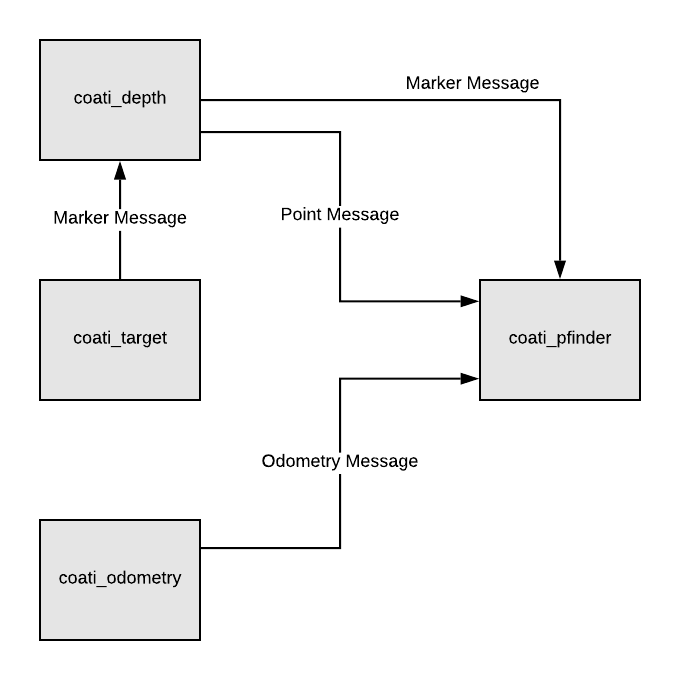
\includegraphics[width=0.6\linewidth]{PathFinderDiagram.png}
		\caption{Route Planning Node}
		\label{fig:routeplanning}
	\end{figure}

	Route planning takes input from the other three custom nodes and determines a route that should carry it toward the target. The current proposed solution is currently to create a potential field where positive vectors that repel the robot are attached to all obstacles while a large negative vector is attached to the target location.
	
	As the route node receives more information about the robot moving through the environment should apply transformations to all of the contained vectors to keep them up to date with where they would be as the robot changes position in the environment. 
	
	This will also require having a method to remove un-necessary or repetitive vectors. This will be easy to implement with the target vector as the targets will have identification values meaning that the current target can be verified. With obstacles this will be more difficult, and initially vectors will probably simply expire after a certain amount of time. 
	
	The route planning software should provide a direction vector to the robot controlling node 10 times every second. There is no need for the route to be the optimal route given that the environment is unknown.

	\subsection{Node Diagram}

	\begin{figure}[H]
		\centering
		\includegraphics[width=0.8\linewidth]{NodeDiagram}
		\caption{Project Node Diagram}
		\label{fig:nodediagram}
	\end{figure}


	Through Figure \ref{fig:nodediagram} it can been shown what nodes will be created or used for this project. The diagram displays what node will subscribe to the other nodes, such as the simple target finder node will subscribe to the video processor node to get messages about the target's potential location. Both the TurtleBot and the Flying Robot have two movement nodes, this is to first build a simple movement node on the platform for testing purposes, then the proper and final movement node will be made and implemented on the respective robot. 

	
	\subsection{Mathematical Modeling}
	
		\subsubsection{Flying Robot}
	
		Given that a quad-copter has six degrees of freedom, modeling them is a very difficult task. The AscTec Pelican already has many existing models intended for use with ROS. There is also a large collection of hardware agnostic tools for operating a quad-copter.
	
		\subsubsection{Robot in 3D Space}
		
		The robot itself will need to remember where it is located in its environment. Remembering where targets are located relative to the robot is necessary, and presumably remembering the locations of obstacles will be used as well. Using quaternion vectors relative to the robot will allow for simple transformations on these vectors while using very little computational power \cite{williams2010combining}. ROS contains methods and messages to easily communicate, convert, and apply transformations to quaternions.
	
		\subsubsection{Pose Estimation}
	
		Initially feedback from inertial sensors will be used for pose estimation, but ideally a version of Optical Flow would be used to estimate the position of the robot in 3D space. There are some libraries in OpenCV that have addressed generalized pose estimation in 6 degrees of freedom, but it requires a significant amount of computational power, a higher frame rate than our goal of 10Hz to be used for real time performance, and hundreds of visual odometry measurements must be made in every frame requiring a visually busy background.

	\subsection{Interfacing}
	
	The interfacing of almost all sensors with the on-board computer will be done over USB. Communication between different nodes on the same computer, and any computers off-board the robot, will be done exclusively with ROS messages sent over either internal loops or Wi-Fi.





\section{Equipment}

	\subsection{Equipment Table}
	
	A large number of items are being used in this project, most are arbitrary and may be changed in future iterations. Part way through our project we intend to re-implement the entire solution onto a different platform. A naming convention has been developed for all of our components using a three character code.
	
	The first letter, ascending from A for hardware and descending from Z for software, represents the subsystem or general classification the equipment falls under. The second character represents a generic piece of equipment, and the third is for a particular example that we are using for our project. Any part with the same two first letters should be able to be substituted freely, an example may be two cameras. One camera (CAA) may be used on the Turtlebot as it is built in to the Turtlebot frame, while another (CAB) may be used on the flying robot as it is much lighter. The generic camera (CA-) can refer to any camera which provides the same information to the same nodes. The equipment table is shown in Table \ref{table:equipment}.
	
	\begin{table}
		\small
		\begin{tabular}{|rl|rl|rl|}
			\hline
			\multicolumn{2}{|c|}{\textbf{Purpose}} & \multicolumn{2}{c|}{\textbf{Description}} & \multicolumn{2}{c|}{\textbf{Equipment}} \\ \hline
			A & Ground Based Robot     & A & Robot              & A   & Clearpath Robotics Turtlebot 2    \\
			A & Ground Based Robot     & B & Robot Controller   & A   & Acer Aspire E-11                  \\
			A & Ground Based Robot     & C & Robot Base         & A   & Kobuki Robot Base                 \\
			A & Ground Based Robot     & D & Sensors            & A   & Stepper Motor Feedback            \\
			A & Ground Based Robot     & D & Sensors            & B   & Orbbec Astra Pro Sensors          \\
			A & Ground Based Robot     & D & Sensors            & C   & Gyroscope                         \\ \hline
			B & Flying Robot           & A & Robot              & A   & AscTec Pelican Quadcopter         \\
			B & Flying Robot           & B & Robot Controller   & A   & AscTec Low Level Processor        \\
			B & Flying Robot           & B & Robot Controller   & B   & AscTec High Level Processor       \\
			B & Flying Robot           & B & Robot Controller   & C   & ODROID-XU4                        \\
			B & Flying Robot           & C & Robot Base         & A   & AscTec Pelican Frame              \\ \hline
			C & Camera                 & A & USB Camera         & A   & Orbbec Astra Pro Camera           \\
			C & Camera                 & A & USB Camera         & B   & oCam-1MGN-U Plus                  \\
			C & Camera                 & B & Digital Camera     & A   & AscTec Option 4                   \\ \hline
			D & Offboard Computer      & A & Computer           & A   & Lenovo T520                       \\
			D & Offboard Computer      & A & Computer           & B   & Mathworks VM - ROS Gazebo v3      \\ \hline
			E & Testing Hardware       & A & ArUco Symbol       & 0-9 & Printed Single Digit ArUco Symbol \\
			E & Testing Hardware       & B & Physical Obstacle  & A   & Human                             \\
			E & Testing Hardware       & B & Physical Obstacle  & B   & Box                               \\
			E & Testing Hardware       & B & Physical Obstacle  & C   & Sheet                             \\
			E & Testing Hardware       & C & Motion Tracking    & A   & Reflective Dot                    \\
			E & Testing Hardware       & C & Motion Tracking    & B   & Motion Tracking Cameras           \\
			E & Testing Hardware       & D & Camera Calibration & A   & Printed 7cm Checker Pattern       \\ \hline
			F & Interfacing            & A & Wireless Router    & A   & D-Link 2.4 GHz Router             \\ \hline
			S & Linux Operating System & A & Operating System   & B   & Ubuntu 18.04 Bionic               \\
			S & Linux Operating System & A & Operating System   & K   & Kubuntu (Mathworks) 14.04         \\
			S & Linux Operating System & A & Operating System   & T   & Ubuntu 14.04 Trusty               \\
			S & Linux Operating System & B & Bundled Program    & A   & Generic Loopback Device           \\
			S & Linux Operating System & C & Version Control    & A   & git                               \\ \hline
			T & ROS Service - Custom   & A & Action Services    & A   & Set Goal                          \\ \hline
			U & ROS Service - Standard & A & Action Services    & A   & Trigger                           \\ \hline
			V & ROS Message - Custom   & A & Action Messages    & A   & Goal                              \\
			V & ROS Message - Custom   & A & Action Messages    & B   & Obstacle                          \\ \hline
			W & ROS Message - Standard & A & Sensor Messages    & A   & Image                             \\
			W & ROS Message - Standard & A & Sensor Messages    & B   & PointCloud                        \\
			W & ROS Message - Standard & B & Geometry Messages  & A   & Twist                             \\
			W & ROS Message - Standard & B & Geometry Messages  & B   & Quaternion                        \\
			W & ROS Message - Standard & B & Geometry Messages  & C   & Transform                         \\ \hline
			X & ROS Node - Custom      & A & Depth              & A   & coati\_depth	                 \\
			X & ROS Node - Custom      & B & Path Finder        & A   & coati\_pfinder                     \\
			X & ROS Node - Custom      & B & Odometry           & B   & coati\_odom	                 \\
			X & ROS Node - Custom      & B & Vision             & D   & coati\_target		          \\ \hline
			Y & ROS Node - Standard    & A & Vision             & A   & vision\_opencv                    \\
			Y & ROS Node - Standard    & A & Vision             & B   & image\_pipeline                   \\
			Y & ROS Node - Standard    & B & Coordinates        & A   & tf                                \\
			Y & ROS Node - Standard    & C & Vision             & B   & image\_pipeline                   \\ \hline
			Z & Robot Operating System & A & Operating System   & A   & ROS Indigo Igloo                  \\
			Z & Robot Operating System & A & Operating System   & B   & ROS Melodic Morenia               \\
			Z & Robot Operating System & B & Bundled Program    & A   & Gazebo2                           \\
			Z & Robot Operating System & B & Bundled Program    & B   & Gazebo7                           \\
			Z & Robot Operating System & B & Bundled Program    & C   & catkin                            \\
			Z & Robot Operating System & B & Bundled Program    & D   & RViz                              \\
			Z & Robot Operating System & B & Bundled Program    & E   & rosbag                            \\
			Z & Robot Operating System & B & Bundled Program    & F   & rqt                               \\
			Z & Robot Operating System & C & Client             & A   & roscpp                            \\
			Z & Robot Operating System & C & Client             & B   & rospy                             \\ \hline
		\end{tabular}
		\normalsize
		\caption{Equipment}
		\label{table:equipment}
	\end{table}




	
\section{Verification and Validation} --wasn't an actual section before but I think it should be? Or it could go under results for how we obtained the results???
	
		\subsection{Unit Tests}
	
	When using ROS it is typical to create individual nodes that all execute independent of one another. Using this modular design, it is easy to write an entire node and verify it individually before executing it with the entire system. Verification and validation of the project's nodes will be done prior to implementation in the Gazebo simulation environment. 
	
		\subsection{Gazebo}
	
	Gazebo is a simulation environment that runs nodes that give similar input and output to nodes being executed on a real robot moving around in a real environment. This includes camera feeds, and allows for the insertion of obstacles and ArUco shapes. Testing of custom written nodes were done in Gazebo congruently with unit-tests to ensure that nodes which rely on subscribing to other nodes are behaving as expected before executing code on an actual robot.
	
		\subsection{Camera Tests}
	
	Given that most of the project's custom nodes revolve around transforming camera data to extract information, the ArUco shapes for targets, parallax shift for obstacles, and optical flow for odometry, tests performed with only the camera and OpenCV outside of a node can be created and and executed without being contained within a ROS node. This was useful as one can use OpenCV's feature highlighting capabilities to ensure that the targets and obstacles were being identified while moving a camera through an environment. 
	
		\subsection{Ground Based Robot}
	
	Testing the code on a ground based robot was necessary to ensure that the logic in the movement nodes is sound. Initial testing was done through simply having the robot follow moving targets or turn to face targets that are not head on. As obstacle avoidance was getting developed ensuring that the robot does avoid the obstacles was enough. When the project was sufficiently developed the testing was having the robot avoid obstacles and move towards a target. As the project moved closer to porting to the flying robot, the ground robot was tested to ensure it met the requirement outlined in the SOR. REFFFFF

		\subsection{Flying Robot}
	
	Similar to the ground based robot, verifying the flying robot primarily involved evaluating its behaviour. The behaviour we expected is the all the functionality that was implemented on the ground based robot previously. 
- Once again it is necessary to ensure all requirements are met... 
- limitations of space, ref scope? Real enviro is only indoors.. I'll grab some issues section for this?
If more complex moves are attempted it may become necessary to test this platform using the motion capture equipment that exists in the lab.

	
\section{Results}
	- presentation of results
	- prove we met the requirements

	- we need to get some data points to prove the target and obstacles are found
	- depth readings
	- able to move towards the target? 
	- talk about what happened with the obstacle avoidance and why it doesn't work


\renewcommand{\arraystretch}{2}
\section{Discussion}

	- detailed analysis of how our design did in relation to the requirements
	- I made some tables so we just have discuss why we met some requirements and how we didn't met others, it says every requirement must be touched on so I just made a table for each type of requirement...
	- talk about why some requirements could not be met or only partially met
	- talk about major issues throughout the project
	- recommendations if anyone expands on this project in the future -- recommendation do something more exciting

	\begin{table}
	    \small
		\begin{tabular}{p{2cm} p{8cm} p{2cm} p{3cm}} 
			\hline
			{\textbf{Index}} & {\textbf{Description of Requirement}} & {\textbf{Result}} & {\textbf{Comment}} \\ \hline
FR-01 & The Turtlebot shall move towards a target under control & Met \\
FR-02 & The Turtlebot shall recognize optically an OpenCV's ArUco shape and be able to give information on the location of the target relative to the robot & Met \\
FR-03 & The Turtlebot shall recognize obstacles in its environment and identify where they are relative to itself & Met? \\
FR-04 & The Turtlebot shall be able to make a deviation from its current movement pattern to avoid an obstacle in its path and then return to its pattern & Not Met & Comment on why or saying we comment below \\
FR-05 & The Turtlebot shall be able to identify multiple obstacles and avoid them accordingly & Partially Met & Able to identify multiple obstacles, not avoid them \\
PR-01 & The Turtlebot shall be able to identify and locate OpenCV's ArUco shapes within a 15m radius & Met \\ \hline
        \end{tabular}
        \caption{Summary of Results for the Turtlebot}
        \label{table:turtlbotresults}
    \end{table}

    The requirements for the Turtlebot can be seen in \ref{table:turtlbotresults}. The reason FR-04 was not satisfied on the Turtlebot is the same reason that was discussed in the results section. FR-05 also was not fully satisfied, the Turtlebot was able to recognize multiple obstacles at once and register each as a potential obstacle. It is the same reason, the obstacle avoidance system, why the requirement was not met. 
    The obstacle avoidance system did not met the requirements on either platform.  

	\begin{table}
	    \small
		\begin{tabular}{p{2cm} p{8cm} p{2cm} p{3cm}}
			\hline
			{\textbf{Index}} & {\textbf{Description of Requirement}} & {\textbf{Result}} & {\textbf{Comment}} \\ \hline
FR-01 & The Flying Robot shall move towards a target under control & Not Met \\
FR-02 & The Flying Robot shall recognize optically an OpenCV's ArUco shape and be able to give information on the location of the target relative to the robot & Met \\
FR-03 & The Flying Robot shall recognize obstacles in its environment and identify where they are relative to itself & Not Met \\
FR-04 & The Flying Robot shall be able to make a deviation from its current movement pattern to avoid an obstacle in its path and then return to its pattern & Not Met  \\
FR-05 & The Flying Robot shall be able to identify multiple obstacles and avoid them accordingly & Not Met \\
PR-01 & The Flying Robot shall be able to identify and locate OpenCV's ArUco shapes within a 15m radius & Not Met \\
PR-02 & The Flying Robot should be able to process an image and plot obstacles at a rate of 10 Hz & Not Met \\
PR-03 & The Flying Robot shall be able to navigate an environment and detect up to two obstacles simultaneously & Not Met \\ \hline
		\end{tabular}
		\caption{Summary of Results for the Flying Robot}
		\label{table:uavresults}
    \end{table}


	\begin{table}
	    \small
		\begin{tabular}{p{2cm} p{8cm} p{2cm} p{3cm}}
			\hline
			{\textbf{Index}} & {\textbf{Description of Requirement}} & {\textbf{Result}} & {\textbf{Comment}} \\ \hline
IT-01 & The Gazebo simulator shall be run on a laptop and robots within the simulation will be interfaced through ROS & Met \\
IT-02 & Communication to the Turtlebot will be done through ROS over USB & Met \\
IT-03 & The Flying Robot will be communicating through ROS over WiFi wireless network & Not Met \\
IT-04 & A simple interface, perhaps command line, will allow a user to select a marker as a target to start the robot's movement towards the target and this signal should be received over wireless transmission & Not Met \\ \hline
		\end{tabular}
		\caption{Summary of Results for the Interface Requirements}
		\label{table:interresults}
    \end{table}

	\begin{table}
	    \small
		\begin{tabular}{p{2cm} p{8cm} p{2cm} p{3cm}}
			\hline
			{\textbf{Index}} & {\textbf{Description of Requirement}} & {\textbf{Result}} & {\textbf{Comment}} \\ \hline
SimR-01 & A Gazebo simulation environment which roughly approximates a lab environment with marker placed around will be created & Met- we kinda did this last semester no? \\
SimR-02 & Stationary obstacles will be added to the lab simulation environment and a Turtlebot shall navigate toward markers in the lab while avoiding obstacles & Not Met \\
SimR-03 & An environment with obstacles will be created a Flying Robot shall navigate toward markers in the simulation while avoiding obstacles & Not Met\\ \hline
		\end{tabular}
		\caption{Summary of Results for the Simulation Requirements}
		\label{table:simresults}
    \end{table}

	\begin{table}
	    \small
		\begin{tabular}{p{2cm} p{8cm} p{2cm} p{3cm}}
			\hline
			{\textbf{Index}} & {\textbf{Description of Requirement}} & {\textbf{Result}} & {\textbf{Comment}} \\ \hline 
ImpR-01 & OpenCV programs shall be created that can use a single video stream and identify both markers and obstacles & Met \\ 
ImpR-02 & Prior to testing on the Turtlebot, the program shall be implemented on the gazebo simulation & Met??? \\
ImpR-03 & Usin the robot in the simulation environment the appropriate components, tools, and libraries to interpret and OpenCV stream, make decisions based on the environment, and execute instructions will be developed & Partially Met & Kinda used Gazebo \\
ImpR-04 & The simplest obstacle avoidance algorithm must be implemented on a Turtlebot using ROS & Met \\
ImpR-05 & The obstacle avoidance algorithm used for a Flying Robot will be implemented in a simulation & Not Met \\ \hline
		\end{tabular}
		\caption{Summary of Results for the Implementation Requirements}
		\label{table:impresults}
    \end{table}

	\begin{table}
	    \small
		\begin{tabular}{p{2cm} p{8cm} p{2cm} p{3cm}}
			\hline
			{\textbf{Index}} & {\textbf{Description of Requirement}} & {\textbf{Result}} & {\textbf{Comment}} \\ \hline 
SchR-01 & The first Turtlebot simulation shall be able to operate in a Gazebo environment no later than November \nth{5} & Not Met \\
SchR-02 & The first functional prototype shall be a Turtlebot robot capable of positively identifying a marker, moving towards the marker, and avoiding an obstacle placed in its environment no later than December \nth{18} & Not Met \\
SchR-03 & The first functional prototype shall be capable of identifying a marker, moving towards the marker, and avoiding an obstacle placed in its environment no later than February \nth{18} & Not Met \\
SchR-04 & Data Item Descriptions (DID) to be presented are DID-04: Preliminary Design Specification due November \nth{22}, DID-05: Preliminary Design Review Presentations due November \nth{29}, and the DID-06: Schedule Update is due January \nth{17}. The DID-07: Final Detailed Design Document is due March \nth{21}, the Final Project Presentation, DID-08, is March \nth{28} and the Final Project Demonstration, DID-09, is on April \nth{9} & Met \\
\\ \hline
		\end{tabular}
		\caption{Summary of Results for the Schedule Requirements}
		\label{table:schresults}
    \end{table}




\section{Conclusion}
The detailed design has been shown for Computer Optics for Analyzing Trajectories in Mostly Unknown, Navigation Denied, Environments (\textsc{coatimunde}). The background outlined how the project has progressed over the year and the motivation behind it. It gave a summary of the previous Data Item Deliverables, such as the Statement of Requirements and the Preliminary Design Document. The design section laid out the final design of the project and how it was implemented. The verification and validation section explained how different aspects of the project were tested throughout the year. The results section showed the final results and how they proved we met the requirements previously outlined. A discussion section gave a detailed analysis of the design in comparison with the requirements and gave recommendations for future expansions of the project.  The final design laid out in this document will also be used in the the Final Project Presentation and the Final Project Demonstration. 

\newpage
\printbibliography

\end{document}    
